\documentclass[tikz]{standalone}
\usepackage{pgfplots}
\pgfplotsset{compat=1.15}
\usepackage{mathrsfs}
\usetikzlibrary{arrows,calc}
\usepackage{tkz-euclide}

\usepackage{fp}
\pagestyle{empty}

\definecolor{AngleClr}{rgb}{0,0.39215686274509803,0}
\definecolor{ShapeClr}{rgb}{0.6,0.2,0}

\begin{document}

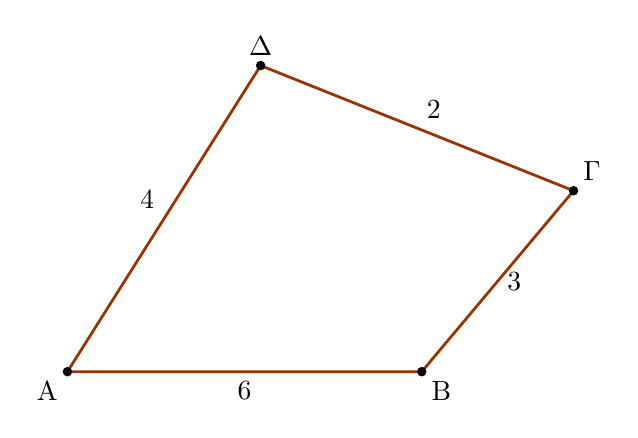
\begin{tikzpicture}[scale=.75]
\tkzSetUpLine[line width=1pt,color=black]
\tkzSetUpPoint[fill=black]

\tkzDefPoint(180:6){A}
\tkzDefPoint(-120:0){B}
\tkzDefPoint(50:4){C}

\begin{scope}[shift=(A)]
\tkzDefPoint(0:3){E}
\end{scope}

\begin{scope}[shift=(C)]
\tkzDefPoint(0:2){Z}
\end{scope}

\tkzInterCC(A,E)(C,Z) \tkzGetPoints{D}{x}

\tkzFillPolygon[fill=white](A,B,C,D)
\tkzDrawPolygon[color=ShapeClr](A,B,C,D)

\tkzDrawPoints[size=3](A,B,C,D)
\tkzLabelPoint[below left](A){$\rm A$}
\tkzLabelPoint[below right](B){$\rm B$}
\tkzLabelPoint[above right](C){$\rm \Gamma$}
\tkzLabelPoint[above](D){$\rm \Delta$}

\tkzLabelSegment(A,B){$6$}
\tkzLabelSegment[right](B,C){$3$}
\tkzLabelSegment[above right](C,D){$2$}
\tkzLabelSegment[above left](D,A){$4$}

\end{tikzpicture}

\end{document}
